\documentclass[11pt]{article}
\usepackage[margin=1in]{geometry}
\usepackage{graphicx}
\usepackage{booktabs}
\usepackage{amsmath}
\usepackage{amssymb}
\usepackage{hyperref}

\title{CS 690S AI Alignment --- Homework 3\\ \large RLHF on CartPole}
\author{Sagnik Chatterjee}
\date{October 21, 2026}

\begin{document}
\maketitle

\section{Setup and results}

The pipeline follows the three parts of the assignment:

\begin{enumerate}
  \item \textbf{Synthetic demonstrations.} A reward-to-go vanilla policy gradient
  (\texttt{vpg.py}) was trained on \texttt{CartPole-v0} for 10 epochs, checkpointing after
  each epoch. These 10 deliberately undertrained policies are the ``demonstrators''.
  \item \textbf{Preference-based reward learning.} One trajectory was rolled out from each
  checkpoint, and 20 random pairs of those trajectories were labelled by \emph{ground-truth}
  return (the higher-return trajectory is preferred). A two-hidden-layer MLP reward network
  $r_\theta : \mathbb{R}^4 \to \mathbb{R}$ (\texttt{utils.py}, \texttt{Net}) scores each state;
  the predicted return of a trajectory is $\hat{J}_\theta(\tau) = \sum_{s_t \in \tau} r_\theta(s_t)$.
  The two predicted returns of a pair are used as the logits of a two-way
  \texttt{CrossEntropyLoss}, i.e.\ the Bradley--Terry model
  \[
    P_\theta(\tau_i \succ \tau_j) \;=\; \frac{\exp \hat{J}_\theta(\tau_i)}
    {\exp \hat{J}_\theta(\tau_i) + \exp \hat{J}_\theta(\tau_j)},
  \]
  trained for 100 epochs with Adam ($\text{lr}=10^{-3}$) and saved to \texttt{reward.params}.
  \item \textbf{RL on the learned reward.} The same policy-gradient algorithm was rerun for 50
  epochs, using \emph{only} $r_\theta$ as the reward signal (the ground-truth reward is never
  seen by the learner), checkpointing into \texttt{rlhf/}.
\end{enumerate}

Measured performance (5 rollouts each, ground-truth return on \texttt{CartPole-v0}, where
200 is the maximum achievable):

\begin{center}
\begin{tabular}{lcc}
\toprule
Policy & 5 rollouts & 20 rollouts \\
\midrule
Best demonstrator (\texttt{synthetic/policy\_checkpoint9}) & 69.2 & 35.2 \\
RLHF policy (\texttt{rlhf/policy\_checkpoint49}) & \textbf{163.0} & --- \\
\bottomrule
\end{tabular}
\end{center}

\noindent Both columns are averages of the ground-truth return over independent rollouts of the
\emph{same} policy; the demonstrator's two numbers differ only because a plain policy gradient at
this stage of training is high-variance, so 5 rollouts is a noisy estimate. The 5-rollout column
is the protocol the assignment specifies, and is the one quoted below; the 20-rollout column is
reported because it is the more reliable estimate, and it only widens the gap in favour of RLHF.

The ten trajectories that actually enter the preference dataset returned
30, 62, 15, 34, 14, 36, 71, 22, 65 and 90 steps respectively, so the best demonstration the
reward model ever saw was 90 steps; the best single demonstrator rollout observed anywhere in these experiments was
115 steps. The learning curve of the RLHF policy over all 50 checkpoints is shown in
Figure~\ref{fig:curve}.

\begin{figure}[h]
  \centering
  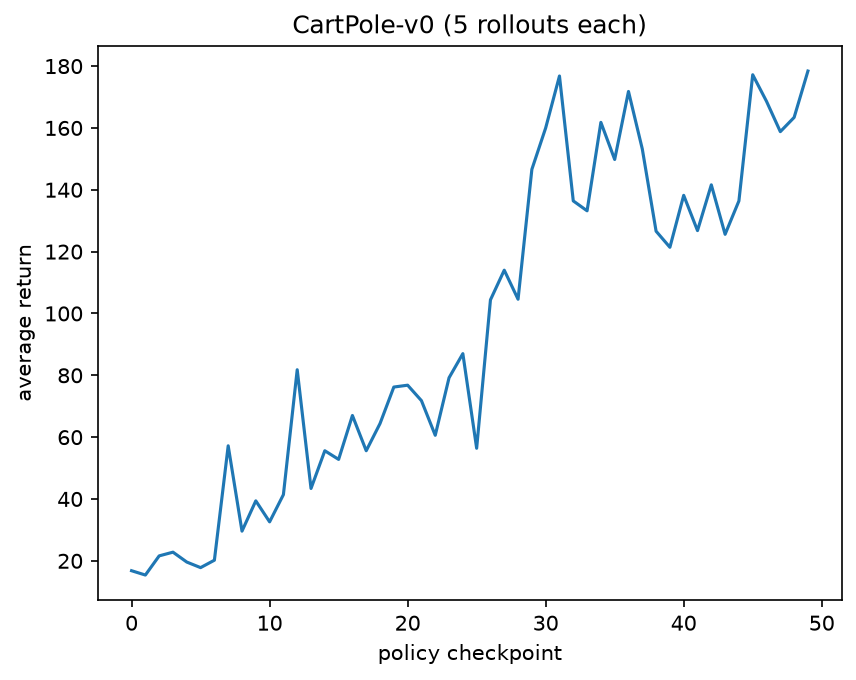
\includegraphics[width=0.75\textwidth]{learning_curve.png}
  \caption{Average ground-truth return (5 rollouts per checkpoint) of the policy trained with
  RL on the \emph{learned} reward function, across all 50 checkpoints, evaluated on
  \texttt{CartPole-v0} (200-step cap, so 200 is optimal). Returns climb from roughly 15 at
  checkpoint 0 to a band of 120--180 over the last 20 checkpoints, peaking around 178. Note that
  the policy being plotted never observed the ground-truth reward during training. The variance
  between neighbouring checkpoints is expected from a plain policy gradient with only 5
  evaluation rollouts per point.}
  \label{fig:curve}
\end{figure}

\section{Questions}

\subsection*{(1) Was the RLHF method able to learn a better policy than the best policy used
to collect training data?}

Yes, and by a wide margin. The best demonstrator (checkpoint 9 of the synthetic run) averages
$69.2$ over 5 rollouts ($35.2$ over 20 rollouts), while the final RLHF policy averages
$163.0$ over the same protocol --- roughly a $2.4\times$ improvement. The RLHF policy also
beats the best \emph{single trajectory} in the preference dataset: no demonstration there
exceeded $90$ steps, and no demonstrator rollout observed anywhere exceeded $115$, whereas the
best RLHF checkpoints average $175$--$178$ out of a maximum of
$200$ (Figure~\ref{fig:curve}) and individual rollouts hit the $200$-step cap, i.e.\ optimal
play. So the learner extrapolated beyond every piece of behaviour it was shown.

\subsection*{(2) Why is it possible to learn a policy much better than the best trajectory in
the training data?}

Because what is learned from the preferences is a \emph{reward function}, not a policy, and the
reward function generalises outside the support of the demonstrations.

\begin{itemize}
  \item \textbf{Preferences are relative, and the ranking carries directional information.}
  A label ``$\tau_i \succ \tau_j$'' does not say ``imitate $\tau_i$''; it says ``move in the
  direction that separates $\tau_i$ from $\tau_j$''. Pairs drawn from checkpoints of different
  quality tell the reward network which states distinguish better behaviour from worse.
  Extrapolating that trend \emph{past}
  the best demonstration is the natural continuation of the gradient it encodes --- the same
  argument as in T-REX (Brown et al., \emph{Extrapolating Beyond Suboptimal Demonstrations via
  Inverse RL from Observations}).
  \item \textbf{The reward decomposes over states, so returns extrapolate over time.}
  Since $\hat{J}_\theta(\tau) = \sum_t r_\theta(s_t)$, and the learned $r_\theta$ turns out to be
  positive at essentially every state the agent visits, each additional timestep of survival adds
  reward. A policy that balances \emph{longer} than any demonstrator therefore automatically earns
  a higher learned return: the reward model never caps out at the best observed return, so the RL
  optimiser is actively rewarded for surpassing the data. Probing the trained network confirms
  this is the operative mechanism --- over the states visited by the ten demonstrators,
  $r_\theta$ has mean $0.57$ and is positive on $91\%$ of them, and on a sweep of the
  $(x,\theta)$ plane it stays in $[0.31, 1.24]$ and is positive everywhere.
  \item \textbf{The reward model does not need to recover the true reward's \emph{shape}.}
  Notably, $r_\theta$ is \emph{not} a recovered copy of the ground-truth reward: it does not rank
  states by how upright the pole is (its correlation with $|\theta|$ over that sweep is
  $\approx 0$, and it scores a tilted, off-centre state slightly \emph{higher} than a centred
  upright one). What the preferences taught it is the much cruder fact that occupying states at all
  is worth roughly $+0.7$ to $+1.2$ per step --- which, because CartPole terminates on failure, is
  behaviourally equivalent to the true reward for the purpose of optimisation. This is a useful
  reminder that a reward model can induce optimal behaviour while still being a poor
  \emph{explanation} of what the ground-truth objective rewards.
  \item \textbf{RL supplies its own fresh experience.} The policy-gradient learner interacts
  with the real environment and generates states the demonstrators never visited. It is not
  limited to the training distribution the way a purely offline imitation method is; it only
  needs the reward model to rank those new states sensibly.
\end{itemize}

The flip side is that this is extrapolation, and it is only safe while the learned reward stays
accurate off-distribution. If the policy drifts far enough from the demonstration support,
the reward model can be exploited (reward hacking) --- CartPole is simple and low-dimensional
enough (4-D state, obvious structure) that the extrapolation holds here.

\subsection*{(3) How is RLHF different from Inverse RL or behavioral cloning?}

\textbf{Behavioral cloning (BC)} is supervised learning on state--action pairs: it fits
$\pi_\phi(a \mid s)$ to match the demonstrator by maximising $\log \pi_\phi(a_t \mid s_t)$ over
the dataset. There is no reward, no environment interaction, and no notion of ``better than''.
Its explicit target is to \emph{reproduce} the demonstrator, so the demonstrator's performance
is a ceiling. It also suffers from covariate shift: small errors push the agent into states
absent from the data, where it has no supervision (the DAgger problem).

\textbf{Classical Inverse RL} does recover a reward function, but under the assumption that the
demonstrations are (near-)optimal --- typically by matching feature expectations or maximum
entropy. The learned reward is the one that \emph{rationalises the demonstrator}, so a policy
that optimises it converges back to roughly demonstrator-level behaviour. It is also typically
expensive: many formulations require solving the forward RL problem in an inner loop.

\textbf{RLHF} differs on three axes:
\begin{itemize}
  \item \emph{Supervision signal.} Comparisons/rankings between behaviours, not action labels
  and not an optimality assumption. Humans are far better at judging ``which of these two is
  better'' than at demonstrating optimal control or writing down a reward.
  \item \emph{What is learned.} A reward model (Bradley--Terry over trajectory returns), which
  is then optimised by a standard RL algorithm. The policy is the product of \emph{optimisation},
  not of imitation.
  \item \emph{Ceiling.} Because the data is explicitly labelled with \emph{relative} quality and
  can come from deliberately suboptimal behaviour, RLHF can rank and then exceed everything it
  was shown. BC and standard IRL are both anchored to the demonstrator.
\end{itemize}

In this assignment a ground-truth-return oracle stands in for the human labeller, which is
exactly the standard synthetic-preference setup: it isolates the algorithmic question from
human-annotation noise. A practical RLHF system would also need to handle noisy, inconsistent,
and sometimes mistaken human labels.

\subsection*{(4) What would have happened if Inverse RL or behavioral cloning were run on the
same trajectories used for RLHF?}

Both would have produced a policy that is \emph{at best} as good as the demonstrations, i.e.\ an
average return somewhere in the 20--60 range, and plausibly worse.

\begin{itemize}
  \item \textbf{Behavioral cloning} would have been trained on an undifferentiated mixture of all
  ten checkpoints --- including checkpoint 0, which barely balances the pole for $\sim 30$ steps.
  BC has no way to tell good data from bad: every state--action pair is treated as a target to
  match. The result would be a policy near the \emph{average} of the demonstrators, roughly
  $30$--$40$ return, which is worse than just copying the best checkpoint. Compounding error
  under covariate shift would likely drag it lower still. Note also that the trajectories stored
  here are \emph{observation-only} (\texttt{generate\_rollout} records states, not actions), so
  plain BC could not even be run on this dataset without re-collecting actions.
  \item \textbf{Inverse RL} would recover a reward function that explains this mixture as if it
  were optimal behaviour. Since the mixture contains many early failures (pole falling after
  20--30 steps), the inferred reward would treat ``drop the pole fairly quickly'' as rational,
  and optimising it would reproduce mediocre behaviour rather than surpass it. The demonstrator
  distribution becomes the target, so there is nothing to extrapolate along.
\end{itemize}

The key difference is the preference labels. The same ten trajectories carry a strong learning
signal once they are \emph{ranked}: the ranking reveals which direction in behaviour space is
``better'', and that direction can be followed beyond the data. Treated as things to copy, the
same trajectories are a mediocre dataset and bound the learner to mediocre performance.

\end{document}
